
\clearpage
\cleardoublepage

\chapter{Related Work}
\label{chap:related_work}
As we traverse the intricate terrain of geospatial data analysis in the realm of global Earth system models,
it becomes of utmost importance to have a comprehensive grasp of the existing methodologies and advancements.
This chapter starts on an extremely thorough investigation of the seminal works and groundbreaking research that
have laid the foundation for the utilization of Convolutional Neural Networks (CNNs) in geospatial analysis.
It delves deeply into the evolution of convolutional architectures, highlighting their application in various scientific
fields beyond conventional image processing, encompassing their transformative potential in climatology, oceanography, and meteorology.
By thoroughly analyzing both Euclidean and non-Euclidean convolutional operations, this discussion aspires to offer a contextual framework
for the current research within the broader domain of deep learning investigation, highlighting the importance of adapting and optimizing CNNs
to effectively exploit the complex, multidimensional nature of geospatial data.
@TODO: review [usman]
\section{Convolutions On Euclidean Space}
\subsection{Convolutional Neural Networks (CNN)}
With the advent of deep learning models, convolutional neural networks were developed primarily for solving the vision related tasks. These architectures are now being embraced across various scientific disciplines for the purpose of data analysis, owing to their utilization of convolutions.
In case of the climate data studies where the observations obtained are subjected to spatial mapping via latitudes and longitudes, forming a grid like structure which could be analyzed by the Convolutional neural networks.
Computer vision pertains to the examination of images, which are mostly multi-channel grids. In the case of RBG images, an image could be described as three grids stacked together, each grid containing information about a specific color (Red, Blue, Green) for a pixel. Similarly, geospatial data which is relevant under the same latitudes and longitudes mapping could be stacked together for the analysis harnessing the Convolutional Neural Networks (CNN).

Below are the main advatages of using convolutional neural networks:
\begin{itemize}
    \item \textbf{Learnable Kernels}\\
          Convolutional neural networks possess the inherent capability to process \textbf{grid-format} data using 2D convolutions, as presented in \cite{LeChun_5}, where they were used for the MNIST dataset\cite{deng2012mnist} for the hand written digit classification.
          The convolution layer of the network is facilitated by \textbf{learnable kernels}. The learning of the kernels happens due to back propagation as in the gradient base-learning.
          These kernels traverse the image, capturing distinctive features within the gridded data and generating feature maps for subsequent layers in the network to further extract relevant features.

\end{itemize}
\begin{itemize}
    \item \textbf{Preserves Spatial Context }\\
          A drawback of fully connected architectures is their complete disregard for the input's topology. The presentation order of input variables can be arbitrary without affecting the training outcome. Images possess a strong \textbf{local structure}, where spatially adjacent variables or pixels exhibit high \textbf{correlation}. These local correlations contribute to the well-known benefits of extracting and combining local features prior to recognizing spatial objects, such as edges or corners. Convolutional Networks enforce the extraction of local features
          by confining the receptive fields of hidden units to be local \cite{LeChun_5}.
\end{itemize}

\begin{itemize}
    \item \textbf{Shift Invariance}\\
          In the convolutional networks, the property of shift invariance is achieved through the weight configurations being replicated across space\cite{LeChun_5}.

\end{itemize}
\begin{itemize}
    \item \textbf{Tolerance of Transformation }\\
          Convolutional layers possess a core characteristic where the output of the feature map will undergo a shift of the same magnitude as the input image, but remain unaltered in all other aspects. This particular attribute forms the foundation for the resilience exhibited by convolutional networks against shifts and distortions encountered in the input data\cite{LeChun_5}.
          The precise location of a detected feature diminishes in significance once it has been identified. The only relevant aspect is its approximate position in relation to other features \cite{LeChun_5}.
\end{itemize}


\begin{figure}[h]
    \centering
    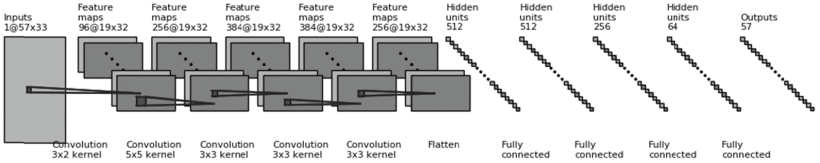
\includegraphics[width=1.0\linewidth]{figures/chapter-4/han3-2955957-large.png}
    \caption{Architecture for estimating subsurface temperatures in Pacific Ocean (Source \cite{8913542}) }
    \label{fig:architecture-pacific-ocean}
\end{figure}

Due to the above mentioned properties, convolutional neural networks are used for the geospatial data as the Figure ~\ref{fig:architecture-pacific-ocean} shows an architecture which is used for predicting the subsurface temperature.
This model is using the grid-format data for capturing the advanced features through the high dimensional data \cite{8913542}. The usage of the convolutional neural networks is also to reduce the time of feature engineering \cite{8913542}.


\subsection{Convolutional Block Attention Module (CBAM)}
Even though the convolutional neural networks perform well in capturing the features in the planar data (grid) but this comes with a cost of creating deeper architectures as VGG16\cite{simonyan2015deep} with more than hundred million trainable parameters, VGG16 was utilized for image recognition task \cite{simonyan2015deep}.

There has been attraction to attention mechanism, which tries to focus on the features extracted by the convolutions which have more data activity.
Since convolution operations combine cross-channel and spatial information to extract informative features, The method proposed \cite{woo2018cbam} focuses on enhancing meaningful features along these two principal dimensions: channel and spatial axes \cite{woo2018cbam}.
The utilization of the attention was separated into two parts first the learning of the channel attention and after that learning the spatial attention \cite{woo2018cbam}. This removes the unwanted clutter and focuses on only the relevant features \cite{woo2018cbam}.

\begin{figure}[h]
    \centering
    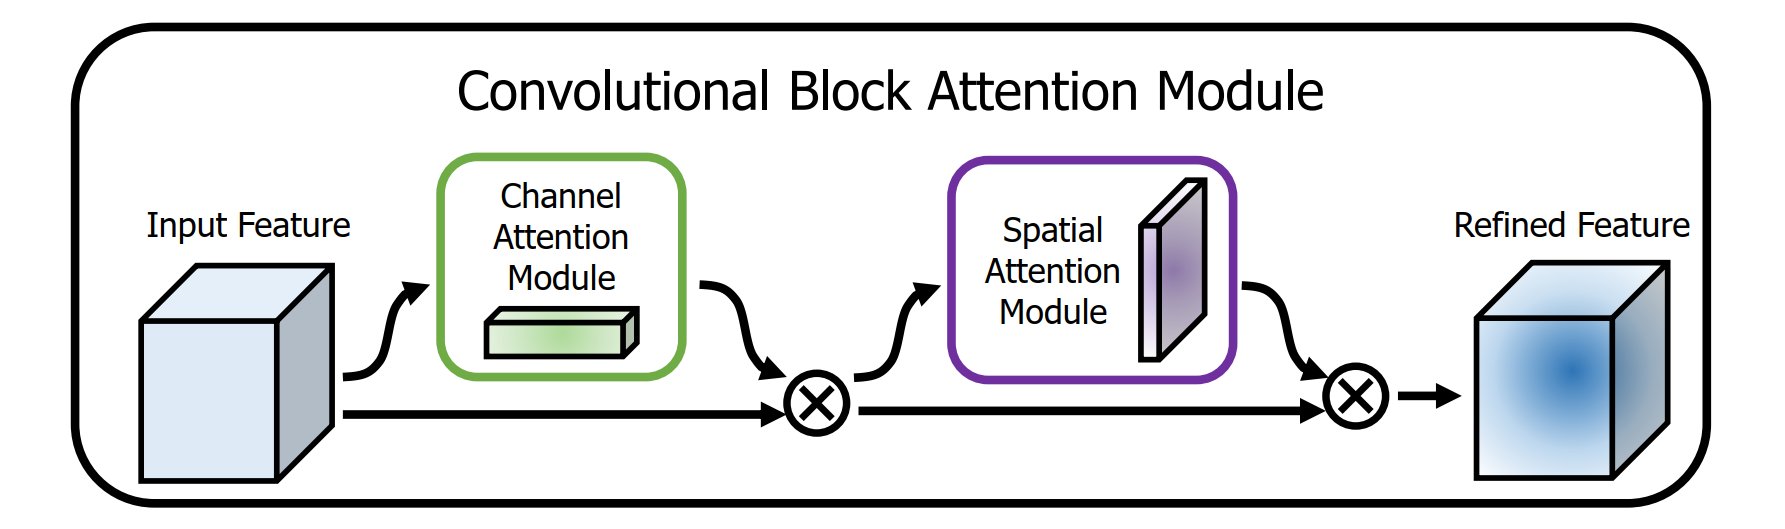
\includegraphics[width=1.0\linewidth]{figures/chapter-4/CBAM.png}
    \caption{Convolutional Block Attention Module (CBAM) (Source \cite{woo2018cbam}) }
    \label{fig:cbam-image}
\end{figure}

Figure ~\ref{fig:cbam-image} depicts the two types of attention modules which applied in a sequential manner for boosting the performance of the network\cite{woo2018cbam}.

In the context of analyzing geospatial data, the utilization of CBAM has proven to enhance performance \cite{mao2023reconstructing}.
The CBAM module utilization is also happening for nowcasting the precipitation \cite{trebing2021smaatunet}. Both \cite{mao2023reconstructing} \cite{trebing2021smaatunet} are being used on the smaller regions of the globe.

\subsection{U-Net}

U-Net architecture was first used in the segmentation task for the medical images. The name of the architecture is because of its shape. This deep neural network architecture incorporates both the encode and the decoder parts in the same architecture. As mentioned the usage of the proposed architecture was to give each pixel of the image a class.


\begin{figure}[h]
    \centering
    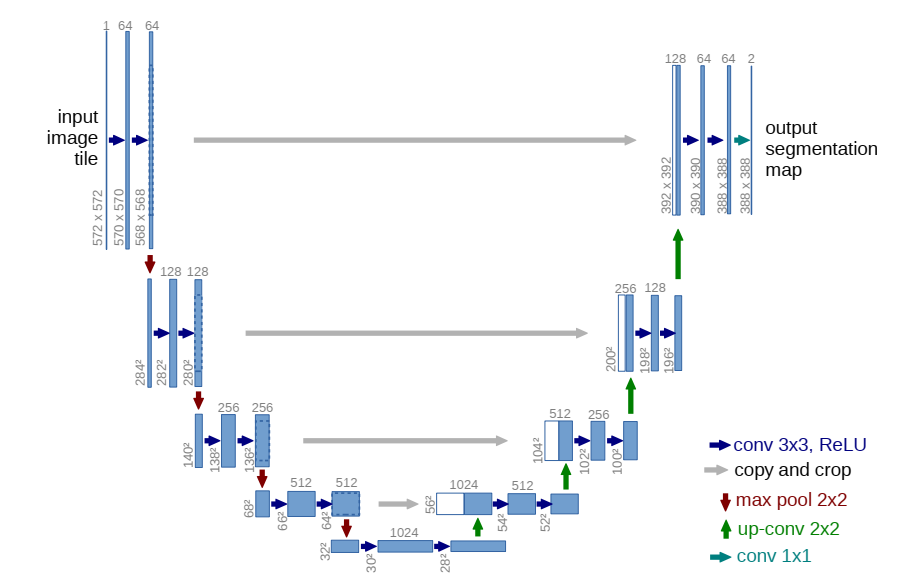
\includegraphics[width=1.0\linewidth]{figures/chapter-4/unet.png}
    \caption{Original U-Net proposed for the segmentation of the medical images (Source \cite{ronneberger2015unet}) }
    \label{fig:unet}
\end{figure}

As seen in figure ~\ref{fig:unet}, the major feature of the architecture is that the left hand side is the contraction part and the right hand side in the expansion \cite{ronneberger2015unet}. Each of the contraction and the expansion block of the network is utilizing double convolutional layers \cite{ronneberger2015unet}.
In order to achieve localization, the upsampled output is combined with high resolution features obtained from the contracting path. Subsequently, a convolution layer is employed to acquire the ability to construct a more accurate output, utilizing the information provided \cite{ronneberger2015unet}.

For the geospatial analysis, rather than giving each pixel a class actual values are generated for the data under consideration \cite{trebing2021smaatunet}. A combination of U-Net and ConvLSTM are used, the U-Net is used to predict the heatwave intensity under the observed area of South China sea \cite{rs15164068}.

\section{Convolutions on Non-Euclidean Space}
The convolutional neural networks were initially designed for the capturing patterns in the Euclidean 2D space, for images which are in the format of a grid. The data is represented in equirectangular grids, which aligns with the nature of the image data.
Currently, various scientific fields are encountering problems related to accurately representing their data. In the past, data in these fields was primarily analyzed by projecting it onto a Euclidean plane before conducting further analysis.
With the advent of Geometric machine learning, new techniques are being developed to study data on non-euclidean spaces. This approach brings the data closer to its actual representation.
Thus it provides the mechanism to perform convolutional operation on the non-euclidean spaces and manifolds

\subsection{Spherical CNN}

In a planar image, the arrangement of patterns can be altered through movement, whereas in the case of patterns on the sphere, their movement is characterized by a three-dimensional rotation rather than a translation \cite{cohen2018spherical}.
The substitution of the definition of cross-correlation or convolution necessitates the substitution of filter translations by rotations \cite{cohen2018spherical}.

The set of movements on the sphere could be described in a three-dimensional space, known as 3D rotations and they can be described as a manifold SO(3) \cite{cohen2018spherical}. When spherical correlation or convolution is performed, the resulting feature map are to be regarded as a signal on SO(3) rather than a signal on the sphere, $S^2$ \cite{cohen2018spherical}.
The efficient implementation of the $S^2$ and SO(3) correlation can be achieved through the utilization of generalized FFT algorithms \cite{cohen2018spherical}.

The feature maps in the spherical convolution are generated at a rotation $R \in SO(3)$ by the inner product of a filter and a feature map using the rotation $R$ \cite{cohen2018spherical}.
For computing the spherical convolutions data and the filters are considered as continuous functions $f: S^2 \rightarrow  \mathbb{R}^K $, K is the number of channels\cite{cohen2018spherical}.
Spherical CNNs provide the rotational equivariance.

The calculation of the spherical convolution can be carried out in the harmonic space by executing matrix multiplications involving the harmonic coefficients of the spherical signal and the filter. This approach is particularly advantageous due to the familiarity of deep learning practitioners with utilizing GPUs to efficiently perform matrix multiplications \cite{towardsdatascienceGeometricDeep}.

\begin{itemize}
    \item \textbf{Parameterized Differential Operators }\\
          This technique performs effective convolutions on the manifolds which are approximated by the underlying meshes.In order to achieve these convolutions, the convolutional kernels that can be learned are reparameterized into a linear combination of differential operators. In this technique the differential operators of different order take place of the cross correlation linear operators to find local features \cite{jiang2019spherical}. This approach is could also be used for modeling the climate data.
          For the experimentation, U-Net based architecture is deployed.

\end{itemize}


\subsection{Spherical U-Net}
This architecture comes from the medical field, where the model is designed for studying the brain as sphere. While the spherical CNN \cite{cohen2018spherical} considers the data as continuous functions, this approach depends on the discretization of the sphere using the icosahedron structure and generating the uniform sphere by hierarchically adding new vertices \cite{zhao2019spherical}.
In \cite{zhao2019spherical}, \textbf{Direct Neighbor (DiNe)} filters and convolutions are proposed which use the consistent neighborhood orders on the spherical space\cite{zhao2019spherical}. Such an approach could be used for the geo science related machine learning tasks. The issue for such tasks would be the discretization of the geo-spatial data on the sphere.


\begin{figure}[h]
    \centering
    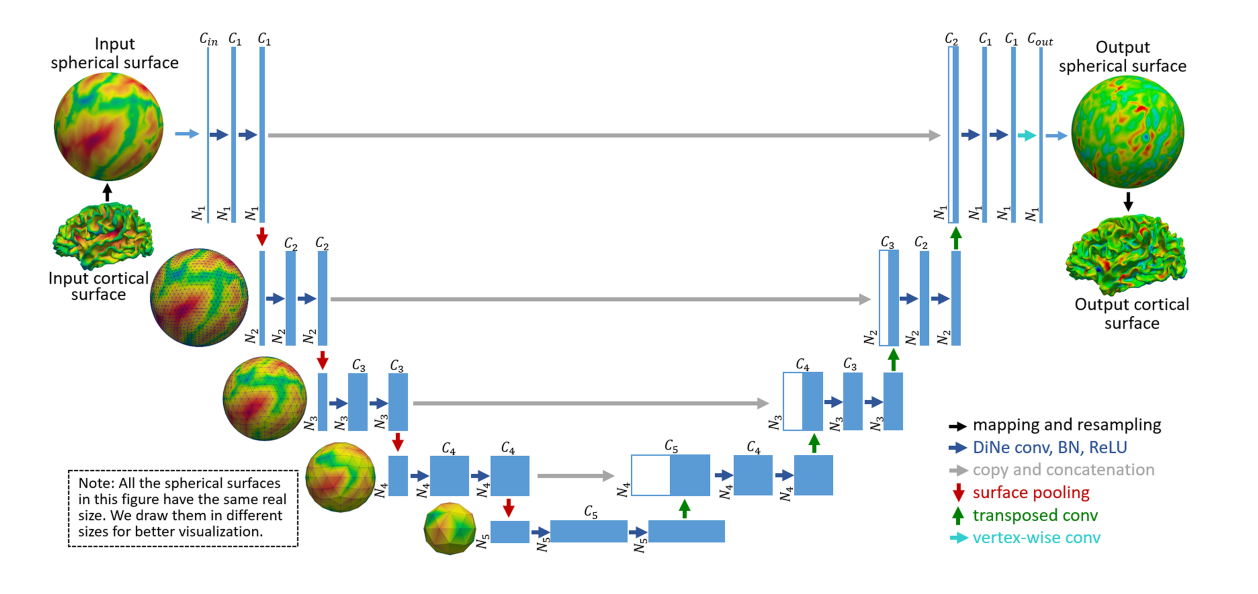
\includegraphics[width=1.0\linewidth]{figures/chapter-4/spherical_unet.png}
    \caption{Spherical U-Net for the brain cortical surface (Source \cite{zhao2019spherical}) }
    \label{fig:spherical-unet}
\end{figure}

\section{Sphere2Vec}
This is an encoder model which is trying to mitigate the distortion of distance that arises from the map projections. This method can encode spherical coordinates by abstaining from the distortions of the map projections and spherical to Euclidean distance approimation errors \cite{mai2023sphere2vec}. 2D Discrete Fourier Transform basis are used in the technique of multi-scale encoding to measure the accurate distances on the sphere \cite{mai2023sphere2vec}. While \cite{mai2023sphere2vec} also argues about the incapability of 2D and NeRF-style 3D location encoders to correctly find spherical distances.